% Options for packages loaded elsewhere
\PassOptionsToPackage{unicode}{hyperref}
\PassOptionsToPackage{hyphens}{url}
%
\documentclass[
  9pt,
  ignorenonframetext,
  aspectratio=169]{beamer}
\usepackage{pgfpages}
\setbeamertemplate{caption}[numbered]
\setbeamertemplate{caption label separator}{: }
\setbeamercolor{caption name}{fg=normal text.fg}
\beamertemplatenavigationsymbolsempty
% Prevent slide breaks in the middle of a paragraph
\widowpenalties 1 10000
\raggedbottom
\setbeamertemplate{part page}{
  \centering
  \begin{beamercolorbox}[sep=16pt,center]{part title}
    \usebeamerfont{part title}\insertpart\par
  \end{beamercolorbox}
}
\setbeamertemplate{section page}{
  \centering
  \begin{beamercolorbox}[sep=12pt,center]{part title}
    \usebeamerfont{section title}\insertsection\par
  \end{beamercolorbox}
}
\setbeamertemplate{subsection page}{
  \centering
  \begin{beamercolorbox}[sep=8pt,center]{part title}
    \usebeamerfont{subsection title}\insertsubsection\par
  \end{beamercolorbox}
}
\AtBeginPart{
  \frame{\partpage}
}
\AtBeginSection{
  \ifbibliography
  \else
    \frame{\sectionpage}
  \fi
}
\AtBeginSubsection{
  \frame{\subsectionpage}
}
\usepackage{lmodern}
\usepackage{amssymb,amsmath}
\usepackage{ifxetex,ifluatex}
\ifnum 0\ifxetex 1\fi\ifluatex 1\fi=0 % if pdftex
  \usepackage[T1]{fontenc}
  \usepackage[utf8]{inputenc}
  \usepackage{textcomp} % provide euro and other symbols
\else % if luatex or xetex
  \usepackage{unicode-math}
  \defaultfontfeatures{Scale=MatchLowercase}
  \defaultfontfeatures[\rmfamily]{Ligatures=TeX,Scale=1}
\fi
\usetheme[]{Berkeley}
\usecolortheme{dove}
\usefonttheme{structurebold}
% Use upquote if available, for straight quotes in verbatim environments
\IfFileExists{upquote.sty}{\usepackage{upquote}}{}
\IfFileExists{microtype.sty}{% use microtype if available
  \usepackage[]{microtype}
  \UseMicrotypeSet[protrusion]{basicmath} % disable protrusion for tt fonts
}{}
\makeatletter
\@ifundefined{KOMAClassName}{% if non-KOMA class
  \IfFileExists{parskip.sty}{%
    \usepackage{parskip}
  }{% else
    \setlength{\parindent}{0pt}
    \setlength{\parskip}{6pt plus 2pt minus 1pt}}
}{% if KOMA class
  \KOMAoptions{parskip=half}}
\makeatother
\usepackage{xcolor}
\IfFileExists{xurl.sty}{\usepackage{xurl}}{} % add URL line breaks if available
\IfFileExists{bookmark.sty}{\usepackage{bookmark}}{\usepackage{hyperref}}
\hypersetup{
  pdftitle={Testes de hipótese},
  pdfauthor={Frederico Bertholini},
  hidelinks,
  pdfcreator={LaTeX via pandoc}}
\urlstyle{same} % disable monospaced font for URLs
\newif\ifbibliography
\usepackage{color}
\usepackage{fancyvrb}
\newcommand{\VerbBar}{|}
\newcommand{\VERB}{\Verb[commandchars=\\\{\}]}
\DefineVerbatimEnvironment{Highlighting}{Verbatim}{commandchars=\\\{\}}
% Add ',fontsize=\small' for more characters per line
\usepackage{framed}
\definecolor{shadecolor}{RGB}{248,248,248}
\newenvironment{Shaded}{\begin{snugshade}}{\end{snugshade}}
\newcommand{\AlertTok}[1]{\textcolor[rgb]{0.94,0.16,0.16}{#1}}
\newcommand{\AnnotationTok}[1]{\textcolor[rgb]{0.56,0.35,0.01}{\textbf{\textit{#1}}}}
\newcommand{\AttributeTok}[1]{\textcolor[rgb]{0.77,0.63,0.00}{#1}}
\newcommand{\BaseNTok}[1]{\textcolor[rgb]{0.00,0.00,0.81}{#1}}
\newcommand{\BuiltInTok}[1]{#1}
\newcommand{\CharTok}[1]{\textcolor[rgb]{0.31,0.60,0.02}{#1}}
\newcommand{\CommentTok}[1]{\textcolor[rgb]{0.56,0.35,0.01}{\textit{#1}}}
\newcommand{\CommentVarTok}[1]{\textcolor[rgb]{0.56,0.35,0.01}{\textbf{\textit{#1}}}}
\newcommand{\ConstantTok}[1]{\textcolor[rgb]{0.00,0.00,0.00}{#1}}
\newcommand{\ControlFlowTok}[1]{\textcolor[rgb]{0.13,0.29,0.53}{\textbf{#1}}}
\newcommand{\DataTypeTok}[1]{\textcolor[rgb]{0.13,0.29,0.53}{#1}}
\newcommand{\DecValTok}[1]{\textcolor[rgb]{0.00,0.00,0.81}{#1}}
\newcommand{\DocumentationTok}[1]{\textcolor[rgb]{0.56,0.35,0.01}{\textbf{\textit{#1}}}}
\newcommand{\ErrorTok}[1]{\textcolor[rgb]{0.64,0.00,0.00}{\textbf{#1}}}
\newcommand{\ExtensionTok}[1]{#1}
\newcommand{\FloatTok}[1]{\textcolor[rgb]{0.00,0.00,0.81}{#1}}
\newcommand{\FunctionTok}[1]{\textcolor[rgb]{0.00,0.00,0.00}{#1}}
\newcommand{\ImportTok}[1]{#1}
\newcommand{\InformationTok}[1]{\textcolor[rgb]{0.56,0.35,0.01}{\textbf{\textit{#1}}}}
\newcommand{\KeywordTok}[1]{\textcolor[rgb]{0.13,0.29,0.53}{\textbf{#1}}}
\newcommand{\NormalTok}[1]{#1}
\newcommand{\OperatorTok}[1]{\textcolor[rgb]{0.81,0.36,0.00}{\textbf{#1}}}
\newcommand{\OtherTok}[1]{\textcolor[rgb]{0.56,0.35,0.01}{#1}}
\newcommand{\PreprocessorTok}[1]{\textcolor[rgb]{0.56,0.35,0.01}{\textit{#1}}}
\newcommand{\RegionMarkerTok}[1]{#1}
\newcommand{\SpecialCharTok}[1]{\textcolor[rgb]{0.00,0.00,0.00}{#1}}
\newcommand{\SpecialStringTok}[1]{\textcolor[rgb]{0.31,0.60,0.02}{#1}}
\newcommand{\StringTok}[1]{\textcolor[rgb]{0.31,0.60,0.02}{#1}}
\newcommand{\VariableTok}[1]{\textcolor[rgb]{0.00,0.00,0.00}{#1}}
\newcommand{\VerbatimStringTok}[1]{\textcolor[rgb]{0.31,0.60,0.02}{#1}}
\newcommand{\WarningTok}[1]{\textcolor[rgb]{0.56,0.35,0.01}{\textbf{\textit{#1}}}}
\usepackage{graphicx}
\makeatletter
\def\maxwidth{\ifdim\Gin@nat@width>\linewidth\linewidth\else\Gin@nat@width\fi}
\def\maxheight{\ifdim\Gin@nat@height>\textheight\textheight\else\Gin@nat@height\fi}
\makeatother
% Scale images if necessary, so that they will not overflow the page
% margins by default, and it is still possible to overwrite the defaults
% using explicit options in \includegraphics[width, height, ...]{}
\setkeys{Gin}{width=\maxwidth,height=\maxheight,keepaspectratio}
% Set default figure placement to htbp
\makeatletter
\def\fps@figure{htbp}
\makeatother
\setlength{\emergencystretch}{3em} % prevent overfull lines
\providecommand{\tightlist}{%
  \setlength{\itemsep}{0pt}\setlength{\parskip}{0pt}}
\setcounter{secnumdepth}{5}

\title{Testes de hipótese}
\subtitle{Métodos Quantitativos Aplicados à Ciência Política}
\author{Frederico Bertholini}
\date{30.nov.2020}

\begin{document}
\frame{\titlepage}

\begin{frame}[allowframebreaks]
  \tableofcontents[hideallsubsections]
\end{frame}
\hypertarget{vamos-falar-de-surveys}{%
\section{Vamos falar de surveys}\label{vamos-falar-de-surveys}}

\begin{frame}{Vamos falar de surveys}
Questionário

Erros não amostrais

Tipos de surveys

Estrutura
\end{frame}

\hypertarget{teste-de-hipuxf3teses}{%
\section{Teste de hipóteses}\label{teste-de-hipuxf3teses}}

\begin{frame}{Teste de hipóteses}
Probabilidade, incerteza e o mundo normal

Padronização, tabelas, t de student\ldots{}

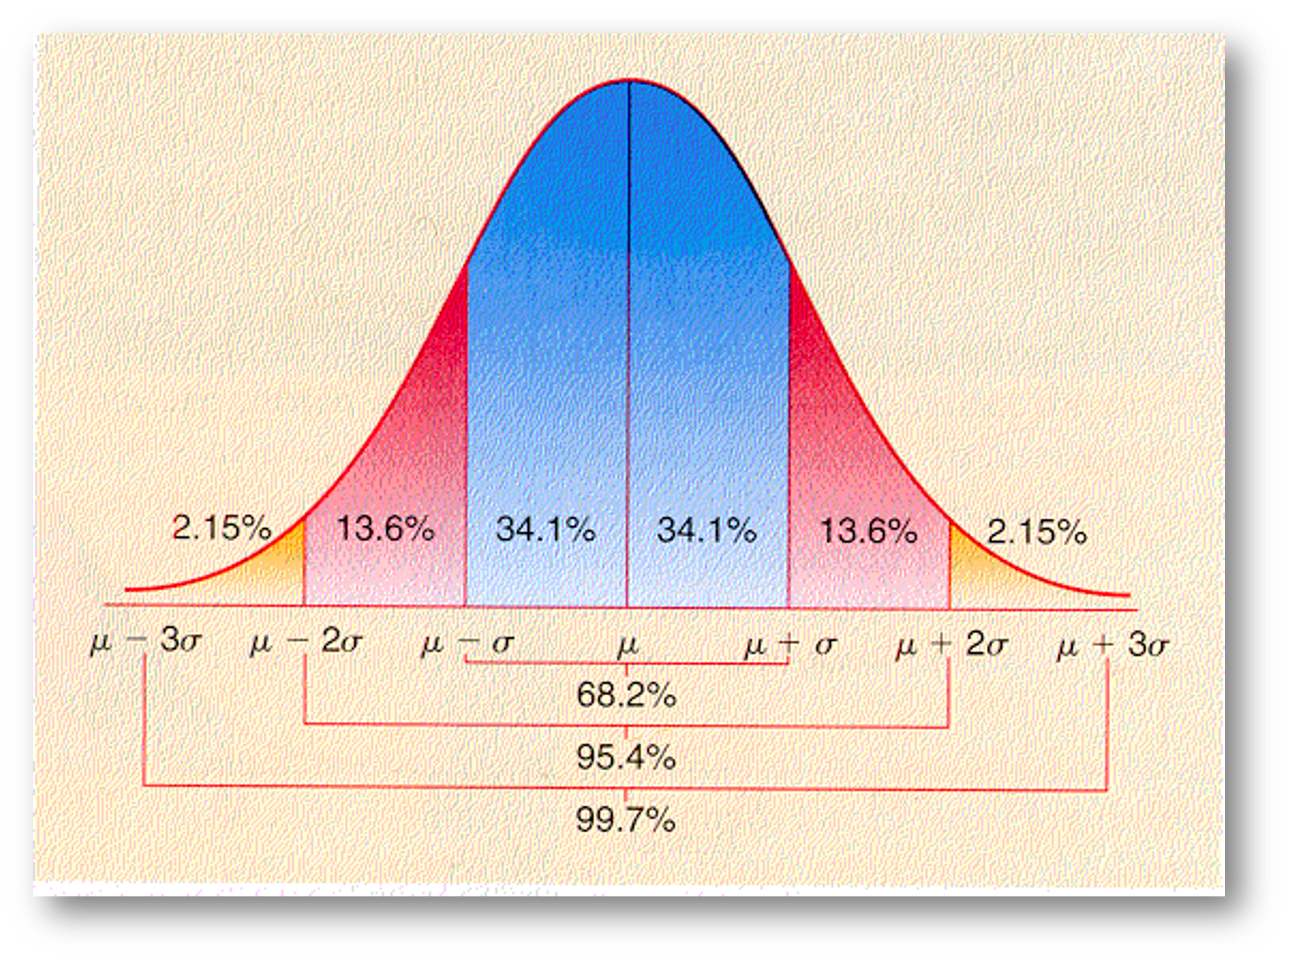
\includegraphics{imgs/normal_percent.png}
\end{frame}

\begin{frame}{Estimativa intervalar}
\protect\hypertarget{estimativa-intervalar}{}
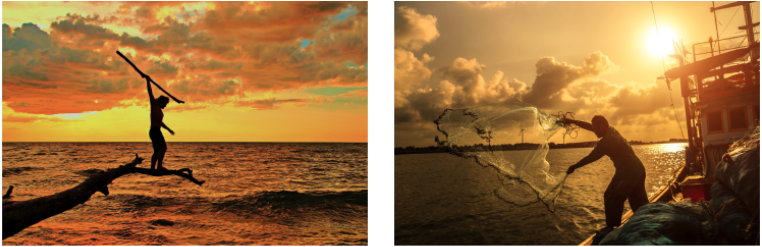
\includegraphics{imgs/point_interval.png}
\end{frame}

\begin{frame}{Teste de hipóteses}
\protect\hypertarget{teste-de-hipuxf3teses-1}{}
Uma \textbf{hipótese} é uma declaração sobre o valor de um parâmetro
desconhecido da população.

Um \textbf{teste de hipótese } consiste em testar duas hipóteses
concorrentes:

-- (1) uma \textbf{hipótese nula} \(H_0\) (pronuncia-se ``H-zero'')

versus

-- (2) uma \textbf{hipótese alternativa} \(H_A\) (também denotada
\(H_1\)).

Geralmente, a hipótese nula é uma afirmação de que ``não há efeito'' ou
``não há diferença de interesse''.

Em muitos casos, a hipótese nula representa o status quo ou uma situação
em que nada de interessante está acontecendo. A hipótese alternativa é a
afirmação que o experimentador ou pesquisador deseja estabelecer ou
encontrar evidências para apoiar. É vista como uma hipótese
``desafiadora'' à hipótese nula \(H_0\).
\end{frame}

\begin{frame}{Erros}
\protect\hypertarget{erros}{}
\begin{enumerate}
\tightlist
\item
  Analogia com um julgamento:
\end{enumerate}

\begin{tabular}{l|l|l}
\hline
Veredito & Verdadeiramente inocente & Verdadeiramente culpado\\
\hline
Inocente & Correto & Erro Tipo II\\
\hline
Culpado & Erro Tipo I & Correto\\
\hline
\end{tabular}

.

\begin{enumerate}
\setcounter{enumi}{1}
\tightlist
\item
  Nossos testes:
\end{enumerate}

\begin{tabular}{l|l|l}
\hline
Decisão & H0 verdadeiro & HA verdadeiro\\
\hline
Não rejeita H0 & Correto & Erro Tipo II\\
\hline
Rejeita H0 & Erro Tipo I & Correto\\
\hline
\end{tabular}
\end{frame}

\hypertarget{suxf3-existe-um-tipo-de-teste}{%
\section{Só existe um tipo de
teste?}\label{suxf3-existe-um-tipo-de-teste}}

\begin{frame}{Só existe um tipo de teste?}
Ao testar hipóteses, você segue este padrão:

Etapa 1: \textbf{Calcular \(\delta\)} É com isso que você se preocupa: a
diferença de médias, a média, a mediana, a proporção, a diferença de
proporções etc. Você está testando para ver se esse número é
significativamente diferente de zero (ou de algum outro número) .

Etapa 2: \textbf{inventar o mundo onde \(\delta\) é nulo.} Simule como
seria o mundo se não houvesse diferença entre os dois grupos, ou se não
houvesse diferença nas proporções, ou se o valor médio fosse um número
específico.

Etapa 3: \textbf{observe \(\delta\) no mundo nulo.} Coloque a
estatística da amostra no mundo nulo e veja se ela se encaixa bem.

Etapa 4: \textbf{calcule a probabilidade de que \(\delta\) poderia
existir em um mundo nulo.} Este é o seu valor p, ou a probabilidade de
ver um \(\delta\) pelo menos tão alto em um mundo onde não há efeito.

Etapa 5: \textbf{decida se \(\delta\) é estatisticamente significativo.}
Escolha algum padrão de evidência ou limite para decidir se há provas
suficientes para rejeitar o mundo nulo. Os limites padrão (do menos ao
mais rigoroso) são 0,1, 0,05 e 0,01.
\end{frame}

\begin{frame}{Estrutura geral do teste}
\protect\hypertarget{estrutura-geral-do-teste}{}
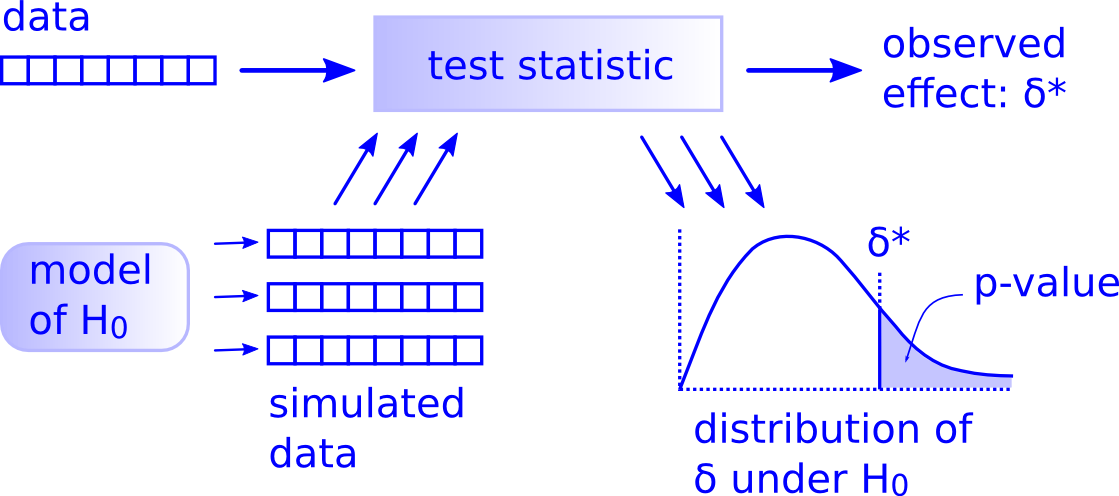
\includegraphics{imgs/there_is_only_one_test.png}
\end{frame}

\begin{frame}[fragile]{``Existe apenas um teste'' com infer}
\protect\hypertarget{existe-apenas-um-teste-com-infer}{}
\begin{enumerate}
\tightlist
\item
  \texttt{specify()} especifica as variáveis e interesse em seu quadro
  de dados.
\item
  \texttt{hypothesize()} hipotetiza a hipótese nula \(H_0\). Em outras
  palavras, defina um ``modelo para o universo'' supondo que \(H_0\)
  seja verdadeiro.
\item
  \texttt{generate()} re-amostra assumindo que \(H_0\) é verdadeiro. Em
  outras palavras, \emph{simula} dados assumindo que \(H_0\) é
  verdadeiro.
\item
  \texttt{calculate()} calcula a \emph{estatística de teste} de
  interesse, tanto para os dados observados quanto para seus dados
  \emph{simulados}.
\item
  \texttt{visualize\ ()} visualiza a \emph{distribuição nula} resultante
  e calcula o \emph{\(p\)-valor} comparando a distribuição nula com a
  estatística de teste observada.
\end{enumerate}

Uma vez que você entenda essa estrutura geral, poderá entender
\emph{qualquer} teste de hipótese. Em uma postagem de blog famosa, o
cientista da computação Allen Downey chamou isso de
\href{http://allendowney.blogspot.com/2016/06/there-is-still-only-one-test.html}{``Há
apenas um teste''}.
\end{frame}

\begin{frame}[fragile]{Pacote infer}
\protect\hypertarget{pacote-infer}{}
Realizar inferência estatística usando uma gramática coerente com o
tidyverse framework.

O pacote é centrado em 4 verbos principais, complementados com muitos
utilitários para visualizar e extrair valor de seus resultados:

\begin{itemize}
\tightlist
\item
  \texttt{specify()} permite que você especifique a variável, ou relação
  entre as variáveis, na qual você está interessado.
\item
  \texttt{hypothesize()} permite que você declare a hipótese nula.
\item
  \texttt{generate()} permite gerar dados que refletem a hipótese nula.
\item
  \texttt{calculate()} permite que você calcule uma distribuição de
  estatísticas a partir dos dados gerados para formar a distribuição
  nula.
\end{itemize}
\end{frame}

\begin{frame}[fragile]{Nível de significância}
\protect\hypertarget{nuxedvel-de-significuxe2ncia}{}
\begin{Shaded}
\begin{Highlighting}[]
\NormalTok{bootstrap\_distribution \textless{}{-}}\StringTok{ }\NormalTok{pennies\_sample }\OperatorTok{\%\textgreater{}\%}\StringTok{ }
\StringTok{  }\KeywordTok{specify}\NormalTok{(}\DataTypeTok{response =}\NormalTok{ year) }\OperatorTok{\%\textgreater{}\%}\StringTok{ }
\StringTok{  }\KeywordTok{generate}\NormalTok{(}\DataTypeTok{reps =} \DecValTok{1000}\NormalTok{) }\OperatorTok{\%\textgreater{}\%}\StringTok{ }
\StringTok{  }\KeywordTok{calculate}\NormalTok{(}\DataTypeTok{stat =} \StringTok{"mean"}\NormalTok{)}
\NormalTok{bootstrap\_distribution}
\end{Highlighting}
\end{Shaded}

\begin{verbatim}
# A tibble: 1,000 x 2
   replicate  stat
       <int> <dbl>
 1         1 1991.
 2         2 1997.
 3         3 1994.
 4         4 1996.
 5         5 1996.
 6         6 1992 
 7         7 1993.
 8         8 1995.
 9         9 1996.
10        10 1995.
# ... with 990 more rows
\end{verbatim}
\end{frame}

\begin{frame}[fragile]{}
\protect\hypertarget{section}{}
\begin{Shaded}
\begin{Highlighting}[]
\NormalTok{percentile\_ci \textless{}{-}}\StringTok{ }\NormalTok{bootstrap\_distribution }\OperatorTok{\%\textgreater{}\%}\StringTok{ }
\StringTok{  }\KeywordTok{get\_confidence\_interval}\NormalTok{(}\DataTypeTok{level =} \FloatTok{0.95}\NormalTok{, }\DataTypeTok{type =} \StringTok{"percentile"}\NormalTok{)}
\NormalTok{percentile\_ci}
\end{Highlighting}
\end{Shaded}

\begin{verbatim}
# A tibble: 1 x 2
  lower_ci upper_ci
     <dbl>    <dbl>
1    1991.    1999.
\end{verbatim}
\end{frame}

\begin{frame}[fragile]{}
\protect\hypertarget{section-1}{}
\begin{Shaded}
\begin{Highlighting}[]
\KeywordTok{visualize}\NormalTok{(bootstrap\_distribution) }\OperatorTok{+}\StringTok{ }
\StringTok{  }\KeywordTok{shade\_confidence\_interval}\NormalTok{(}\DataTypeTok{endpoints =}\NormalTok{ percentile\_ci)}
\end{Highlighting}
\end{Shaded}

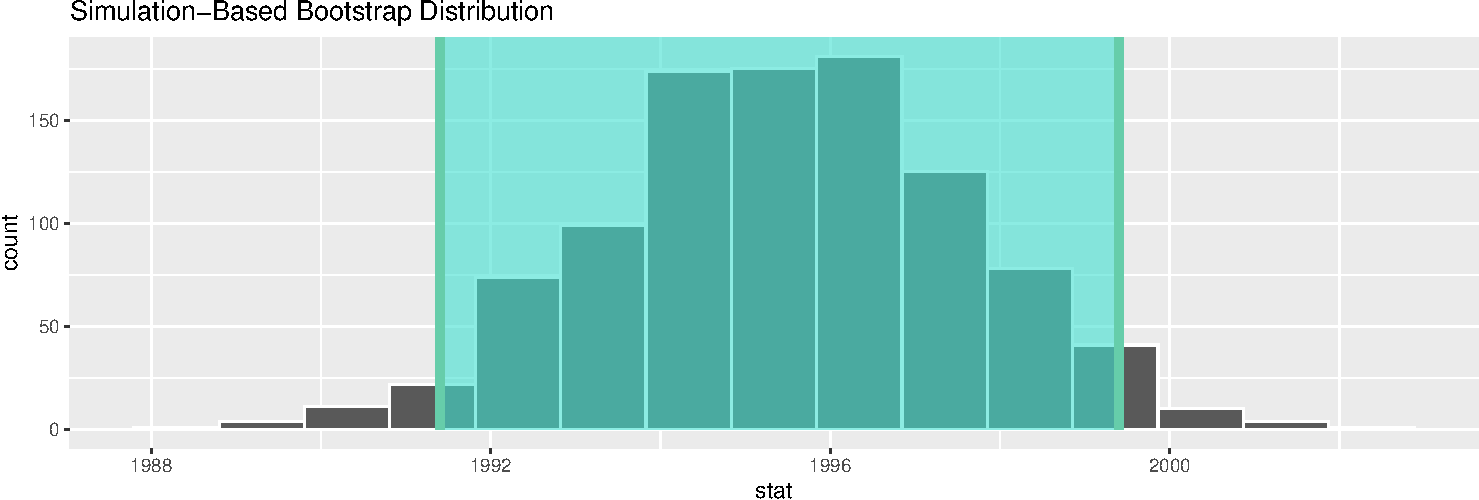
\includegraphics{aula_10_files/figure-beamer/unnamed-chunk-5-1.pdf}
\end{frame}

\begin{frame}{Pacote srvyr}
\protect\hypertarget{pacote-srvyr}{}
Live coding
\end{frame}

\hypertarget{testes}{%
\section{Testes}\label{testes}}

\begin{frame}[fragile]{unilateral}
\protect\hypertarget{unilateral}{}
Testando a hipótese de que a média é maior que 7

\begin{Shaded}
\begin{Highlighting}[]
\CommentTok{\# Média dfe}
\NormalTok{media\_turma \textless{}{-}}\StringTok{ }\NormalTok{dfe }\OperatorTok{\%\textgreater{}\%}\StringTok{ }
\StringTok{  }\KeywordTok{specify}\NormalTok{(media }\OperatorTok{\textasciitilde{}}\StringTok{ }\OtherTok{NULL}\NormalTok{) }\OperatorTok{\%\textgreater{}\%}
\StringTok{  }\KeywordTok{calculate}\NormalTok{(}\DataTypeTok{stat =} \StringTok{"mean"}\NormalTok{)}

\NormalTok{null\_media \textless{}{-}}\StringTok{ }\NormalTok{dfe }\OperatorTok{\%\textgreater{}\%}\StringTok{ }
\StringTok{  }\KeywordTok{specify}\NormalTok{(media }\OperatorTok{\textasciitilde{}}\StringTok{ }\OtherTok{NULL}\NormalTok{) }\OperatorTok{\%\textgreater{}\%}
\StringTok{  }\KeywordTok{hypothesize}\NormalTok{(}\DataTypeTok{null =} \StringTok{"point"}\NormalTok{, }\DataTypeTok{mu =} \DecValTok{70}\NormalTok{) }\OperatorTok{\%\textgreater{}\%}
\StringTok{  }\KeywordTok{generate}\NormalTok{(}\DataTypeTok{reps =} \DecValTok{1000}\NormalTok{) }\OperatorTok{\%\textgreater{}\%}
\StringTok{  }\KeywordTok{calculate}\NormalTok{(}\DataTypeTok{stat =} \StringTok{"mean"}\NormalTok{)}

\NormalTok{null\_media }\OperatorTok{\%\textgreater{}\%}\StringTok{ }\KeywordTok{get\_p\_value}\NormalTok{(}\DataTypeTok{obs\_stat =}\NormalTok{ media\_turma, }\DataTypeTok{direction =} \StringTok{"greater"}\NormalTok{)}
\end{Highlighting}
\end{Shaded}

\begin{verbatim}
# A tibble: 1 x 1
  p_value
    <dbl>
1       0
\end{verbatim}
\end{frame}

\begin{frame}[fragile]{Resultado gráfico}
\protect\hypertarget{resultado-gruxe1fico}{}
\begin{Shaded}
\begin{Highlighting}[]
\KeywordTok{visualize}\NormalTok{(null\_media) }\OperatorTok{+}\StringTok{ }\KeywordTok{shade\_p\_value}\NormalTok{(}\DataTypeTok{obs\_stat =}\NormalTok{ media\_turma, }\DataTypeTok{direction =} \StringTok{"greater"}\NormalTok{)}
\end{Highlighting}
\end{Shaded}

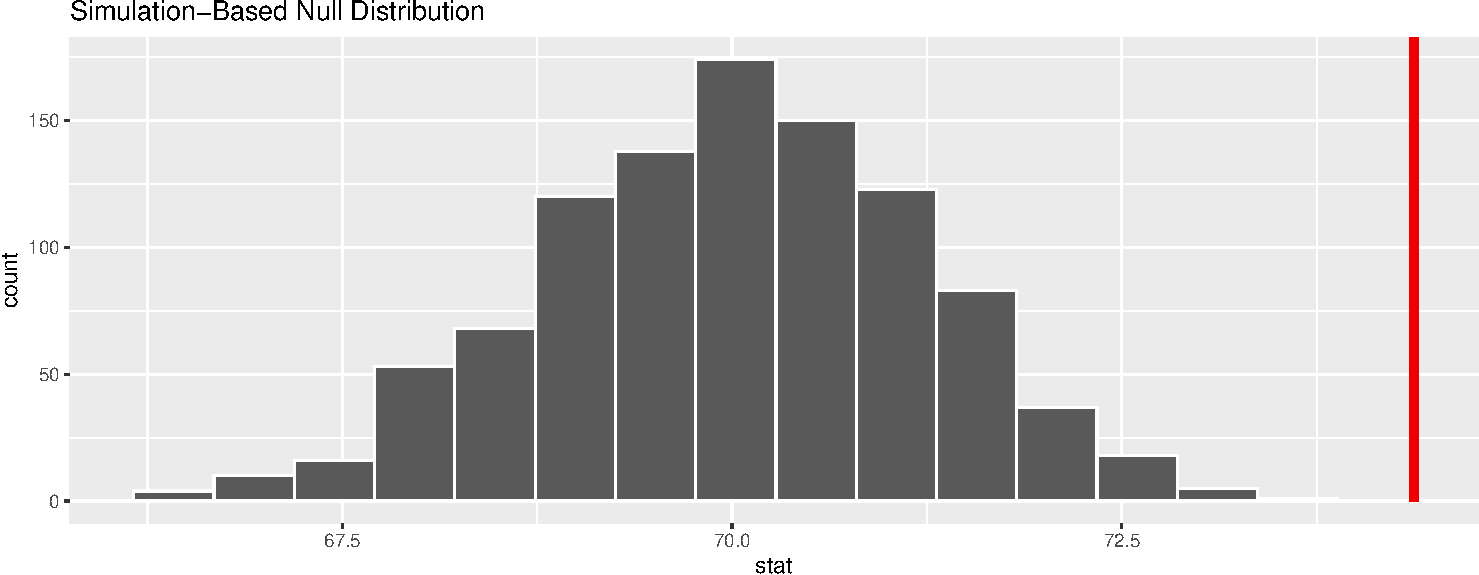
\includegraphics{aula_10_files/figure-beamer/unnamed-chunk-7-1.pdf}
\end{frame}

\begin{frame}{Diferenças de proporções}
\protect\hypertarget{diferenuxe7as-de-proporuxe7uxf5es}{}
Live coding
\end{frame}

\begin{frame}{Teste Diferença de médias}
\protect\hypertarget{teste-diferenuxe7a-de-muxe9dias}{}
Live coding
\end{frame}

\begin{frame}[fragile]{usando t\_test}
\protect\hypertarget{usando-t_test}{}
\begin{Shaded}
\begin{Highlighting}[]
\NormalTok{t\_test\_results \textless{}{-}}\StringTok{ }\NormalTok{dfe }\OperatorTok{\%\textgreater{}\%}
\StringTok{  }\KeywordTok{t\_test}\NormalTok{(}
    \DataTypeTok{formula =}\NormalTok{ media }\OperatorTok{\textasciitilde{}}\StringTok{ }\OtherTok{NULL}\NormalTok{,}
    \DataTypeTok{alternative =} \StringTok{"greater"}\NormalTok{,}
    \DataTypeTok{mu =} \DecValTok{70}
\NormalTok{  )}
\NormalTok{t\_test\_results}
\end{Highlighting}
\end{Shaded}

\begin{verbatim}
# A tibble: 1 x 6
  statistic  t_df  p_value alternative lower_ci upper_ci
      <dbl> <dbl>    <dbl> <chr>          <dbl>    <dbl>
1      3.49    59 0.000464 greater         72.3      Inf
\end{verbatim}
\end{frame}

\begin{frame}[fragile]{ANOVA}
\protect\hypertarget{anova}{}
Vários grupos e uma medida quantitativa

Princípio: Teste F:
\(\Huge\frac{\text{Variância entre grupos}}{\text{Variância dentro dos grupos}}\)

\begin{Shaded}
\begin{Highlighting}[]
\NormalTok{ANOVAtest \textless{}{-}}\StringTok{ }\KeywordTok{aov}\NormalTok{(}\DataTypeTok{data=}\NormalTok{dfe,}\DataTypeTok{formula =}\NormalTok{ media }\OperatorTok{\textasciitilde{}}\StringTok{ }\NormalTok{turma)}

\KeywordTok{summary}\NormalTok{(ANOVAtest)}
\end{Highlighting}
\end{Shaded}

\begin{verbatim}
            Df Sum Sq Mean Sq F value Pr(>F)  
turma        2    703   351.5   4.116 0.0214 *
Residuals   57   4867    85.4                 
---
Signif. codes:  0 '***' 0.001 '**' 0.01 '*' 0.05 '.' 0.1 ' ' 1
\end{verbatim}
\end{frame}

\begin{frame}[fragile]{Teste de Tukey}
\protect\hypertarget{teste-de-tukey}{}
\begin{Shaded}
\begin{Highlighting}[]
\NormalTok{Tt \textless{}{-}}\StringTok{ }\KeywordTok{TukeyHSD}\NormalTok{(ANOVAtest)}
\NormalTok{Tt}\OperatorTok{$}\NormalTok{turma }\OperatorTok{\%\textgreater{}\%}\StringTok{ }
\StringTok{  }\KeywordTok{as.data.frame}\NormalTok{() }\OperatorTok{\%\textgreater{}\%}\StringTok{ }\KeywordTok{rownames\_to\_column}\NormalTok{() }\OperatorTok{\%\textgreater{}\%}
\StringTok{  }\KeywordTok{mutate}\NormalTok{(}\DataTypeTok{rowname =} \KeywordTok{gsub}\NormalTok{(}\StringTok{"}\CharTok{\textbackslash{}n}\StringTok{"}\NormalTok{,}\StringTok{""}\NormalTok{,rowname)) }\OperatorTok{\%\textgreater{}\%}
\StringTok{  }\NormalTok{knitr}\OperatorTok{::}\KeywordTok{kable}\NormalTok{(}\DataTypeTok{col.names =} \KeywordTok{c}\NormalTok{(}\StringTok{""}\NormalTok{,}\StringTok{"Dif."}\NormalTok{,}\StringTok{"Lim inf"}\NormalTok{,}\StringTok{"Lim sup"}\NormalTok{,}\StringTok{"p{-}valor"}\NormalTok{),}
               \DataTypeTok{digits=}\DecValTok{3}\NormalTok{,}\DataTypeTok{format =} \StringTok{"latex"}\NormalTok{)}
\end{Highlighting}
\end{Shaded}

\begin{tabular}{l|r|r|r|r}
\hline
 & Dif. & Lim inf & Lim sup & p-valor\\
\hline
3joan-3joad & -8.306 & -15.530 & -1.081 & 0.021\\
\hline
5joan-3joad & -5.818 & -12.689 & 1.052 & 0.112\\
\hline
5joan-3joan & 2.487 & -4.580 & 9.555 & 0.676\\
\hline
\end{tabular}
\end{frame}

\end{document}
